\subsection{Passenger Reservation}
\subsubsection{Positive Response}
It is 9.00 in the morning and Tom has already download the mobile application called \textit{myTaxiService} and he has a fixed appointment at 17.00 at "Stazione Centrale of Milano" so he decides to reserve a taxi for the 16.30 to go there. He enters in the apposite section of the application, indicates the source of the journey,the destination, the time of the meeting with the Taxi driver. He also specify the number of passengers that the Taxi will carry. The system, after a few seconds, reply positively to Tom saying that the reservation has been accepted and that the Taxi identification number will be provided 10 minutes before the meeting time.



\subsubsection{Negative Response}
It is 16.00 in the morning and Tom has already download the mobile application called \textit{myTaxiService} and he has a fixed appointment at 17.00 at "Stazione Centrale of Milano" so he decides to reserve a taxi for the 16.30 to go there. He enters in the apposite section of the application, indicates the source of the journey,the destination, the time of the meeting with the Taxi driver. He also specify the number of passengers that the Taxi will carry.
The system immediately replies that the specified meeting time is too close to the actual time and that it is only possible to reserve a taxi for a meeting time at least two hours from the time of reservation. The reservation is canceled.

\begin{figure}[H]
\centering
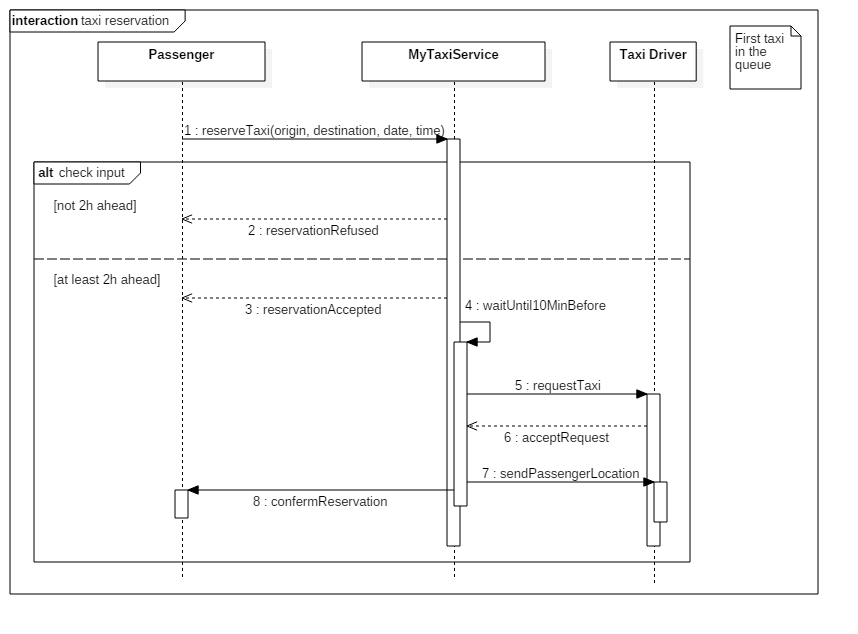
\includegraphics[scale=0.5]{Images/sequence_taxi_reservation}
\end{figure}


